\documentclass[10pt]{article}
\usepackage[a4paper,margin=18mm]{geometry}
\usepackage{amsmath,amssymb,amsthm,mathtools}
\usepackage{graphicx}
\usepackage{microtype}
\usepackage{xcolor}
\usepackage[colorlinks=true,linkcolor=blue!55!black,citecolor=blue!55!black,urlcolor=blue!55!black]{hyperref}

\newtheorem{theorem}{Theorem}
\newtheorem{proposition}[theorem]{Proposition}
\newtheorem{corollary}[theorem]{Corollary}
\newcommand{\R}{\mathbb R}
\newcommand{\Z}{\mathbb Z}
\newcommand{\F}{\mathcal F}
\newcommand{\Cl}{\mathrm{Cl}_{0,n}^{\mathbb C}}
\newcommand{\PW}{\mathrm{PW}}
\newcommand{\supp}{\operatorname{supp}}
\newcommand{\sinc}{\operatorname{sinc}}
\newcommand{\op}{\mathrm{op}}

\title{Stable Sampling for Riesz--Feller Bernstein Spaces\\
\large Explicit RKHS kernels, spacetime reconstruction, and endpoint obstructions}
\author{Candidate substantial partial result for the outlook of arXiv:2405.04989}
\date{13 August 2026}

\begin{document}
\maketitle

\begin{center}
\fbox{\parbox{0.94\linewidth}{\textbf{Status: candidate substantial partial result, likely valid.}
We give the complete $p=2$ RKHS and a stable Whittaker--Shannon reconstruction
of the entire Riesz--Feller spacetime solution from one lattice of boundary
samples.  Two exact bandlimited examples prove that the same-space Hardy
splitting fails at both $p=1$ and $p=\infty$; a bandpass condition repairs the
obstruction.  The general Hardy/BMO endpoint theory remains open.}}
\end{center}

\section{Source outlook and result}

Bernstein and Faustino identify their generalized Bernstein space with
Clifford-valued functions whose ordinary Fourier transform is supported in a
ball, then leave the following two directions on source PDF p.~29
\cite{BF}.

\begin{center}
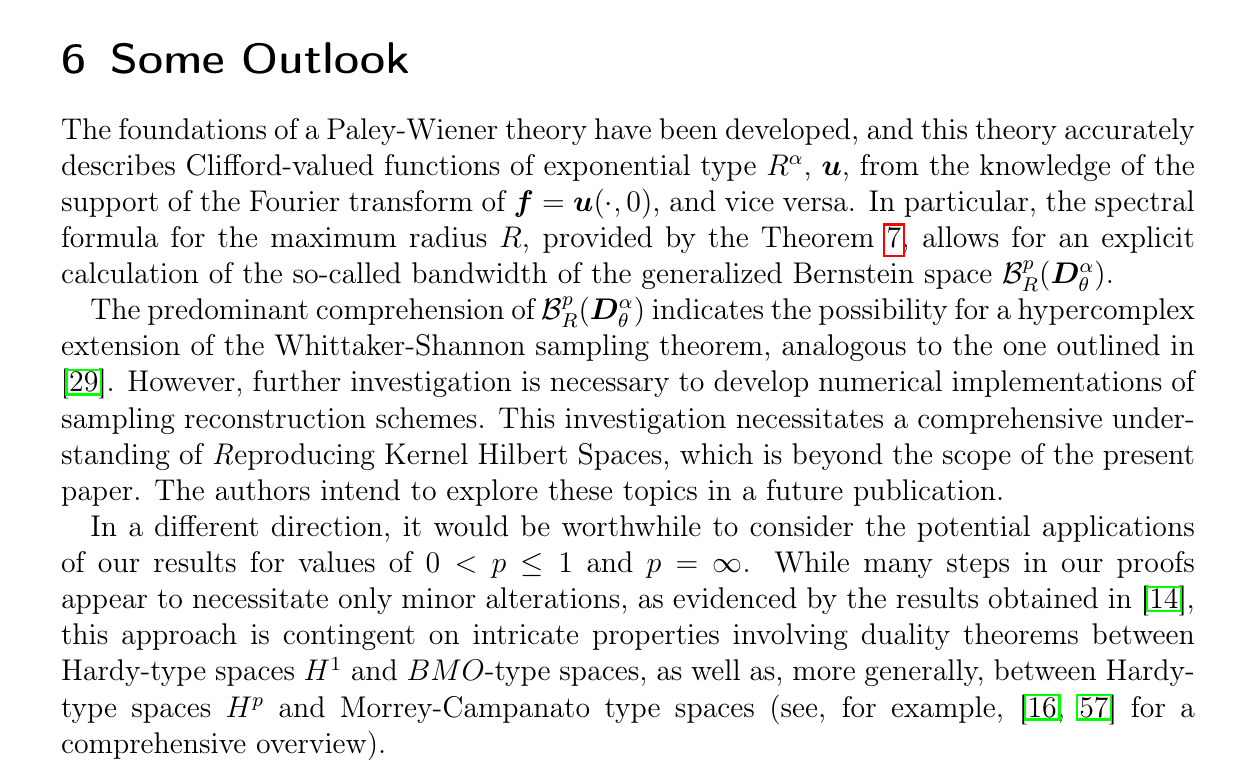
\includegraphics[width=0.91\linewidth]{figures/source_outlook_crop.png}
\end{center}

\noindent\textbf{Exact transcription of the live passages.}
``The predominant comprehension of $\mathcal B_R^p(D_\theta^\alpha)$
indicates the possibility for a hypercomplex extension of the
Whittaker-Shannon sampling theorem, analogous to the one outlined in [29].
However, further investigation is necessary to develop numerical
implementations of sampling reconstruction schemes. This investigation
necessitates a comprehensive understanding of Reproducing Kernel Hilbert
Spaces, which is beyond the scope of the present paper.''  They then write:
``In a different direction, it would be worthwhile to consider the potential
applications of our results for values of $0<p\leq1$ and $p=\infty$.''

We completely answer the Hilbert-space sampling/RKHS part, including stable
finite reconstruction, and prove that a naive endpoint extension is false.
Clifford-valued ball sampling itself is classical \cite{KQS}; the new content
relative to the outlook is the explicit stable propagation through the
Riesz--Feller multiplier and the endpoint diagnosis.

\subsection*{Proof Intuition}

At $p=2$, the difficult analytic work has already been encoded by the source's
Fourier-support theorem.  A function supported in a frequency ball can be
extended by zero to a containing cube.  Its Fourier-series coefficients on
that cube are exactly its samples on the reciprocal lattice.  Applying the
Riesz--Feller solution multiplier term by term produces a spacetime sampling
kernel.  Parseval supplies exact sample stability, while compact frequency
support turns $L^2$ convergence into uniform convergence.

The endpoint issue is concentrated at frequency zero.  The Riesz--Hilbert
multiplier jumps there.  The transforms of $(\sin x/x)^2$ and of the bounded
sine-integral function expose, respectively, a $1/x$ tail and logarithmic
growth.  Removing a neighborhood of zero makes the multiplier smooth and
restores both endpoint bounds by Young's inequality.

\section{The source multiplier and the RKHS}

Let $V=\Cl$ with its finite-dimensional coefficient Hilbert norm.  We use the
source convention
\[
 \widehat f(\xi)=\int_{\R^n}f(x)e^{-ix\cdot\xi}\,dx,
 \qquad
 f(x)=\frac1{(2\pi)^n}\int_{\R^n}\widehat f(\xi)e^{ix\cdot\xi}\,d\xi.
\]
For $\xi\ne0$, put
\[
 \chi_\pm(\xi)=\frac12\left(1\pm\frac{i\xi}{|\xi|}\right).
\]
The source solution with boundary datum $f$ is
$u_f(x,t)=\F^{-1}(M_t\widehat f)(x)$, where
\begin{equation}\label{eq:M}
 M_t(\xi)=
 \begin{cases}
 e^{-t|\xi|^\alpha}\chi_-(\xi),&t>0,\\
 1,&t=0,\\
 e^{-t e^{-i\pi\theta}|\xi|^\alpha}\chi_+(\xi),&t<0.
 \end{cases}
\end{equation}
Here $0<\alpha\leq1$ and $|1-\theta|<\alpha/2$.  Thus
$\cos(\pi\theta)<0$, both scalar factors in \eqref{eq:M} have modulus at
most one in their stated half-spaces, and
\begin{equation}\label{eq:Cchi}
 \sup_{t\in\R,\,\xi\ne0}\|L_{M_t(\xi)}\|_\op\leq C_\chi,
 \qquad
 C_\chi:=\max\{1,\sup_\xi\|L_{\chi_\pm(\xi)}\|_\op\}<\infty.
\end{equation}
The letter $L$ denotes left Clifford multiplication.

Let
\[
 \PW_R^2(V)=\{f\in L^2(\R^n;V):\supp\widehat f\subseteq\overline{B(0,R)}\}.
\]
The source theorem identifies these data with its $p=2$ generalized
Bernstein solutions.

\begin{theorem}[Boundary and spacetime RKHS]\label{thm:rkhs}
The boundary space $\PW_R^2(V)$ is a $V$-valued RKHS with kernel
\begin{align}
 k_R(x,y)
 &=\frac1{(2\pi)^n}\int_{B(0,R)}e^{i(x-y)\cdot\xi}\,d\xi\,I_V \label{eq:ballkernel}\\
 &=\frac{R^{n/2}}{(2\pi)^{n/2}|x-y|^{n/2}}
   J_{n/2}(R|x-y|)I_V, \nonumber
\end{align}
with diagonal value $|B(0,R)|/(2\pi)^n$.

Norm the solution space
$\mathcal H_R=\{u_f:f\in\PW_R^2(V)\}$ by $\|u_f\|_{\mathcal H_R}=\|f\|_2$.
It is an operator-valued RKHS on $\R^n\times\R$ with kernel
\begin{equation}\label{eq:spacekernel}
 \mathbb K((x,t),(y,s))
 =\frac1{(2\pi)^n}\int_{B(0,R)}e^{i(x-y)\cdot\xi}
 L_{M_t(\xi)}L_{M_s(\xi)}^*\,d\xi.
\end{equation}
At $t=s=0$, \eqref{eq:spacekernel} reduces to \eqref{eq:ballkernel}.
\end{theorem}

\begin{proof}
Cauchy--Schwarz on the finite-measure ball makes every boundary evaluation
bounded.  Fourier inversion of the ball indicator gives
\eqref{eq:ballkernel}; the displayed Bessel formula follows by polar
coordinates and has the stated continuous value at zero.

For $z=(x,t)$, define
\[
 E_z\widehat f=\frac1{(2\pi)^n}\int_{B(0,R)}e^{ix\cdot\xi}
 L_{M_t(\xi)}\widehat f(\xi)\,d\xi.
\]
Equation \eqref{eq:Cchi} makes $E_z$ bounded.  Direct computation gives
$E_zE_w^*$ equal to \eqref{eq:spacekernel}; hence that kernel is positive and
reproducing.  Since $u_f(\cdot,0)=f$, the boundary norm defines a genuine
Hilbert norm on the solution space.
\end{proof}

\section{Exact stable sampling of the full solution}

Write $\sinc z=\sin z/z$, with $\sinc0=1$.

\begin{theorem}[Spacetime Whittaker--Shannon formula]\label{thm:sampling}
Let $\Omega\geq R$, $a=\pi/\Omega$, and
$Q_\Omega=[-\Omega,\Omega]^n$.  For $f\in\PW_R^2(V)$ and its source solution
$u_f$, define
\begin{equation}\label{eq:Psi}
 \Psi_{k,t}(x)=\frac{a^n}{(2\pi)^n}
 \int_{Q_\Omega}M_t(\xi)e^{i(x-ak)\cdot\xi}\,d\xi,
 \qquad k\in\Z^n.
\end{equation}
Then
\begin{equation}\label{eq:sampling}
 u_f(x,t)=\sum_{k\in\Z^n}\Psi_{k,t}(x)f(ak).
\end{equation}
The series converges in slice $L^2$, uniformly in $(x,t)$, and at the boundary
\begin{equation}\label{eq:sinc}
 \Psi_{k,0}(x)=\prod_{j=1}^n\sinc(\Omega x_j-\pi k_j).
\end{equation}
Moreover the sample map is an exact scaled isometry:
\begin{equation}\label{eq:parseval}
 \|f\|_2^2=a^n\sum_{k\in\Z^n}|f(ak)|_0^2.
\end{equation}

For a finite $\Lambda\subset\Z^n$, let $u_\Lambda$ be the corresponding
partial sum and
$\tau_\Lambda=(\sum_{k\notin\Lambda}|f(ak)|_0^2)^{1/2}$.  Then
\begin{equation}\label{eq:tails}
 \sup_t\|u_f(\cdot,t)-u_\Lambda(\cdot,t)\|_2
 \leq C_\chi a^{n/2}\tau_\Lambda,
 \qquad
 \sup_{x,t}|u_f(x,t)-u_\Lambda(x,t)|_0
 \leq C_\chi\tau_\Lambda.
\end{equation}
The same bounds hold with $\tau_\Lambda$ replaced by the $\ell^2$ norm of
additive sample noise.
\end{theorem}

\begin{proof}
Extend $\widehat f$ by zero from $B(0,R)$ to $Q_\Omega$.  Its $V$-valued
Fourier series is
\begin{equation}\label{eq:fourierseries}
 \widehat f(\xi)=a^n\sum_{k\in\Z^n}f(ak)e^{-iak\cdot\xi}
 \quad\text{in }L^2(Q_\Omega;V).
\end{equation}
Indeed the Fourier coefficient is $a^nf(ak)$ by Fourier inversion.
Multiplying \eqref{eq:fourierseries} on the left by $M_t$ and inverting gives
\eqref{eq:sampling}; this also explains why the Clifford sample stays on the
right of \eqref{eq:Psi}.  Setting $t=0$ and integrating each coordinate gives
\eqref{eq:sinc}.  Fourier-series Parseval followed by Euclidean Plancherel
gives \eqref{eq:parseval} with no hidden constant.

If $f_\Lambda$ is the boundary partial sum, Parseval gives
$\|f-f_\Lambda\|_2=a^{n/2}\tau_\Lambda$.  Equation \eqref{eq:Cchi} proves the
first estimate in \eqref{eq:tails}.  Every propagated error is
$Q_\Omega$-bandlimited, so Cauchy--Schwarz in Fourier space gives
\[
 \|g\|_\infty\leq
 \left(\frac{|Q_\Omega|}{(2\pi)^n}\right)^{1/2}\|g\|_2
 =a^{-n/2}\|g\|_2.
\]
This cancels the preceding $a^{n/2}$ and proves the uniform estimate.  The
same linear argument applies to any $\ell^2$ noise sequence and also proves
the asserted convergence.
\end{proof}

Thus finite boxes $\Lambda$ provide a directly implementable stable scheme:
precompute the kernels \eqref{eq:Psi}, acquire boundary samples, and certify
the error from the omitted or noisy sample $\ell^2$ norm.

\section{Both naive endpoints fail}

In dimension one, the source's Riesz--Hilbert transform is the classical
Hilbert transform below, times a fixed Clifford generator.  That generator
does not affect integrability or boundedness.

\begin{theorem}[Exact endpoint obstructions]\label{thm:endpoints}
There is a scalar bandlimited $f\in L^1(\R)$ such that $Hf\notin L^1(\R)$,
and a scalar bandlimited $g\in L^\infty(\R)$ such that
$Hg\notin L^\infty(\R)$.  Consequently the source decomposition
$f_\pm=(f\pm Hf)/2$ cannot define the proposed endpoint theory while keeping
both boundary pieces in the same endpoint space.
\end{theorem}

\begin{proof}
Let
\[
 f(x)=\left(\frac{\sin x}{x}\right)^2,
 \qquad
 \widehat f(\xi)=\pi\left(1-\frac{|\xi|}{2}\right)_+.
\]
Thus $f\in L^1$ and is supported in frequency on $[-2,2]$.  Multiplication by
the Hilbert symbol $-i\,\mathrm{sgn}\,\xi$ and direct inversion give
\begin{equation}\label{eq:Hf}
 Hf(x)=\int_0^2\left(1-\frac\xi2\right)\sin(x\xi)\,d\xi
 =\frac1x-\frac{\sin(2x)}{2x^2}.
\end{equation}
Hence $|Hf(x)|\sim1/|x|$, so $Hf\notin L^1$.

For the other endpoint, put
\[
 g(x)=\frac2\pi\int_0^x\frac{\sin s}{s}\,ds.
\]
This function is bounded, and
$\widehat{g'}=2\mathbf1_{[-1,1]}$; therefore the distributional Fourier
support of $g$ is contained in $[-1,1]$ (a possible residual term is supported
at zero).  The Hilbert transform commutes with differentiation, and direct
inversion of $-2i\,\mathrm{sgn}(\xi)\mathbf1_{[-1,1]}$ yields
\[
 (Hg)'(x)=\frac2\pi\frac{1-\cos x}{x}.
\]
Thus, up to an additive constant,
\begin{equation}\label{eq:Hg}
 Hg(x)=\frac2\pi\int_0^x\frac{1-\cos s}{s}\,ds
 =\frac2\pi\log|x|+O(1),
\end{equation}
which is unbounded.
\end{proof}

\begin{proposition}[Bandpass endpoint repair]\label{prop:bandpass}
Fix $0<\rho<R$.  On data with
$\supp\widehat f\subseteq\{\rho\leq|\xi|\leq R\}$, the Riesz--Hilbert
transform is bounded on every $L^p$, $1\leq p\leq\infty$.
\end{proposition}

\begin{proof}
Choose $\eta\in C_c^\infty(\R^n\setminus\{0\})$ equal to one on the stated
annulus.  Then
\[
 Hf=K*f,
 \qquad
 K=\F^{-1}\left[\frac{-i\xi}{|\xi|}\eta(\xi)\right]\in\mathcal S(\R^n).
\]
Young's inequality gives $\|Hf\|_p\leq\|K\|_1\|f\|_p$ at both endpoints and
all intermediate exponents.  Hence the source Hardy splitting is well-defined
on this bandpass subspace.
\end{proof}

\section{Verification, limitations, and novelty}

The verifier checks the exact Parseval constant on $f=(\sin x/x)^2$, tensor
sinc convergence, propagation through a fractional Hardy multiplier, the
uniform tail inequality, and the logarithmic slopes in \eqref{eq:Hf} and
\eqref{eq:Hg}.  All tests pass.  These computations audit constants; the
proofs are analytic.

\textbf{Limitations.}
The cube formula oversamples a ball but is exact.  We do not prove a general
$L^p$ sampling theorem, nor do we replace $L^1$ by $H^1$ or $L^\infty$ by
BMO.  Proposition~\ref{prop:bandpass} is a clean endpoint subspace, not a full
endpoint Paley--Wiener theorem.

\textbf{Bounded novelty audit.}
Cheap run-index searches and focused primary-source searches through 13
August 2026 found no later Riesz--Feller sampling/RKHS follow-up.  The cited
2007 paper already samples Clifford-valued ball-bandlimited boundary
functions with Bessel expansions \cite{KQS}.  We therefore claim only the
explicit operator-valued RKHS, stable boundary-to-spacetime propagation, and
the exact endpoint obstruction/repair in the source's new multiplier setting.

\textbf{Human-review recommendation:} send to an expert in sampling theory and
Clifford harmonic analysis.  Check multiplier handedness, the adjoint in
\eqref{eq:spacekernel}, and whether the broad source outlook warrants a
``substantial partial'' rather than a stronger status.

\begin{thebibliography}{9}
\bibitem{BF}
S.~Bernstein and N.~Faustino,
\emph{Paley--Wiener Type Theorems Associated to Dirac Operators of
Riesz--Feller Type}, arXiv:2405.04989; J. Fourier Anal. Appl. \textbf{31}
(2025), article 52.

\bibitem{KQS}
K.~I. Kou, T.~Qian, and F.~Sommen,
\emph{Sampling with Bessel Functions}, Adv. Appl. Clifford Algebras
\textbf{17} (2007), 519--536.
\end{thebibliography}

\end{document}
